\chapter{Revisão Bibliográfica}

Nesse capítulo será apresentada uma revisão bibliográfica dos tópicos concernentes à acústica interna de dutos circulares, limitamdo-se a modos normais. Os tópicos estão separados em modelos analíticos exatos, modelos analíticos aproximados, trabalhos experimentais, modelos numéricos e trabalhos relacionados ao desenvolvimento e aplicação do método de \textit{lattice} Boltzmann para problemas de acústica.

\section{Modelos Analíticos Exatos} 

A propagação de modos normais (ondas planas) é um problema clássico em acústica e continua tendo importância significativa mediante ao advento de novas tecnologias relacionadas a sistemas de exaustão e sucção. Os dutos são bastante presentes nesses sistemas e. para ondas planas que se propagam no eixo axial $z$, o campo acústico interno é modelado na forma
\begin{equation}
p(z,\omega) = Ae^{ikz} + Be^{-ikz}, 
\end{equation}   
sendo $z$ uma posição axial dentro do duto, $A$ e $B$ constantes no domínio da frequência representando as ondas incidentes e refletidas respectivamente, número de onda $k = \frac{\omega}{c_0}$\simbolo{$k$}{Número de onda}, velocidade do som $c_{0}$ e $\omega$\simbolo{$\omega$}{Frequência angular em radianos} a frequência angular em radianos. Dessa forma o coeficiente de reflexão $R_{z}$ pode ser determinado na forma
\begin{equation}
  R_{z} = \frac{B(\omega)}{A(\omega)}.
\end{equation}

Levando em consideração a terminação do duto, o coeficiente de reflexão nessa região pode ser determinado a partir da formulação apresentada por \citeonline{dalmont2001radiation} na forma
\begin{equation}
  R_{r} = R_{z}e^{2ikz}.
\end{equation}

Segundo \citeonline{dalmont2001radiation} o coeficiente de reflexão na terminação $R_{r}$ pode ser obtido na forma
\begin{equation}
  R_{r} = -|R_{r}|e^{2ikl},
  \label{eq:Rel}
\end{equation} 
sendo $|R_{r}|$ o módulo do coeficiente de reflexão na terminação e $l$ o coeficiente de correção da terminação do duto. Com esses dois parâmetros é possível caracterizar o fenômeno da acústica interna de dutos. Pode-se também obter $|R_{r}|$ segundo a relação de impedâncias
\begin{equation}
    |R_{r}|\simbolo{$R_{r}$}{Coeficiente de reflexão na terminação do duto} =\bigg|\frac{Z_{r} - Z_{0}}{Z_{r} + Z_{0}}\bigg|,
    \label{eq:R}
\end{equation}
sendo $Z_{r}$\simbolo{$Z_{r}$}{Impedância de radiação} a impedância de radiação e $Z_{0}$\simbolo{$Z_{0}$}{Impedância característica do meio} a impedância característica do meio, definida por $Z_{0} = \rho_{0}c_{0}$, tal que $\rho_{0}$ e $c_{0}$ são, respectivamente, as constantes de densidade média do meio\simbolo{$\rho_{0}$}{Densidade média do meio} e velocidade do som\simbolo{$c_{0}$}{Velocidade do som}. E para obter o coeficiente de correção da terminação do duto basta isolar $l$ na Equação \ref{eq:Rel} resultando na equação
\begin{equation}
    l = \frac{1}{k} \arctan\!\left(\frac{Z_{r}}{Z_{0} \, \mathrm{j}\simbolo{$j$}{Unidade imaginária}}\right)
    \label{eq:l}
\end{equation}
sendo o número de onda $k = \frac{\omega}{c_0}$\simbolo{$k$}{Número de onda} e $\omega$\simbolo{$\omega$}{Frequência angular em radianos} a frequência angular em radianos. Nesse sentido, pode-se interpretar $l$ como a quantidade adicional medida a partir da abertura do duto a qual deve propagar a onda incidente antes de ser refletida para o interior do duto com fase invertida. Como cada duto possui um $l$ diferente, para fins de comparação, é preciso tornar essa métrica numa medida adimensional através da normalização pelo raio $a$ do duto, originando $l/a$.

Em relação aos parâmetros discutidos acima, a solução exata para o coeficiente de reflexão e correção da terminação, obtida através da técnica de Wiener-Hopf, para o problema de um duto não flangeado na ausência de escoamento foi proposta por \citeonline{levine1948radiation}. Esse modelo assume um duto semi-infinito com paredes infinitamente finas, fluido invíscido e presença somente de ondas planas. 

 Porém em boa parte das aplicações práticas dutos transportam escoamentos fluidodinâmicos. Para tais circunstâncias, \citeonline{munt1990acoustic} propôs um modelo analítico exato, também baseado na técnica de Wiener-Hopf, em que se considera a presença de um escoamento subsônico no interior do duto. Considera-se nesse modelo as premissas de que o escoamento é uniforme, invíscido e que a camada cisalhante do jato é infinitamente fina. Além disso, o modelo considera a condição de Kutta na borda do duto para lidar com a singularidade da velocidade de partícula nesta região. As Figuras \ref{fig:comp1} e \ref{fig:comp2} apresentam as comparações entre casos com e sem escoamento para um duto não flangeado em termos de $\|R_{r}\|$ e $l/a$.

\begin{figure}[ht!]
\centering
  \begin{tikzpicture}
  \begin{axis}[
  width=.9 \textwidth,
  height=.7 \textwidth,
  xmin=0,
  xmax=1.8,
    ymin=0.4,
    ymax=1.2,
    ytick distance=0.1,
    grid=major, % Display a grid  
  %grid style={dashed,gray!90}, % Set the style
  xlabel = \small{$ka$},
  ylabel = \small{$|R_{r}|$},
  y tick label style={/pgf/number format/.cd,%
          scaled y ticks = false,
          set decimal separator={,},
          fixed},
      x tick label style={/pgf/number format/.cd,%
          scaled x ticks = false,
          set decimal separator={,},
          fixed}%
  ]
 \addplot[color=black, thick] table[x index=0,y index=1] {dados/outros_dados/abs_r_LS.txt};
 \addplot[color=black, dashed] table[x index=0,y index=1] {dados/outros_dados/abs_r_munt.txt};
   
  \end{axis}
  \end{tikzpicture}
  \caption[Magnitudes do coeficiente de reflexão $|R_{r}|$]{Resultados analíticos exatos para magnitude do coeficiente de reflexão $|R_{r}|$ ao final de um duto não flangeado. A linha contínua apresenta o resultado sem escoamento de \citeonline{levine1948radiation} e a linha tracejada apresenta o resultado com escoamento de exaustão para Mach = 0,15 de \citeonline{munt1990acoustic}.}
  \label{fig:comp1}
\end{figure}

\newpage
Como é mostrado na Figura \ref{fig:comp1}, a magnitude do coeficiente de reflexão $|R_{r}|$\simbolo{$|R_{r}|$}{Magnitude do coeficiente de reflexão na terminação do duto} aumenta consideravelmente na presença de um escoamento subsônico. Além disso, pode-se perceber que, em algumas frequências, $|R_{r}|$ torna-se maior do que a unidade, implicando que a amplitude da onda refletida torna-se maior do que a da onda incidente. Este fenômeno ocorre, sobretudo, pela interação entre o escoamento e o campo acústico na borda do duto, a qual transforma energia cinética rotacional em energia acústica, como discutido por \citeonline{peters1993}. Além disso vale ressaltar que o maior valor de $|R_{r}|$ está associado com a frequência de desprendimento de vórtices na saída do duto.

\begin{figure}[ht!]
\centering
  \begin{tikzpicture}
  \begin{axis}[
   width=.9 \textwidth,
  height=.7 \textwidth,
  xmin=0,
  xmax=1.8,
  ymin=0.25,
  ymax=0.65,
  ytick distance=0.05,
  grid=major, % Display a grid  
  %grid style={dashed,gray!90}, % Set the style
  xlabel = \small{$ka$},
  ylabel = \small{$l/a$},
   y tick label style={/pgf/number format/.cd,%
          scaled y ticks = false,
          set decimal separator={,},
          fixed},
      x tick label style={/pgf/number format/.cd,%
          scaled x ticks = false,
          set decimal separator={,},
          fixed}%
  ]
 \addplot[color=black, thick] table[x index=0,y index=1] {dados/outros_dados/loa_LS.txt};
 \addplot[color=black, dashed] table[x index=0,y index=1] {dados/outros_dados/loa_munt.txt};
   
  \end{axis}
  \end{tikzpicture}
  \caption[Coeficientes de correção de terminação $l/a$]{Resultados analíticos exatos para o coeficiente de correção da terminação normalizado pelo raio $l/a$ de um duto não flangeado. A linha contínua apresenta o resultado sem escoamento de \citeonline{levine1948radiation} e a linha tracejada apresenta o resultado com escoamento de Mach = 0,15 de \citeonline{munt1990acoustic}.}
  \label{fig:comp2}
\end{figure}

\newpage
De acordo com a Figura \ref{fig:comp2}, a correção normalizada da terminação $l/a$ torna-se consideravelmente menor do que aquela obtida na ausência de escoamento, sobretudo para baixos números de Helmholtz ($ka$)\simbolo{$ka$}{Número de Helmholtz}. Em outras palavras, para baixas frequências e na presença de um escoamento a onda acústica é refletida em uma região mais próxima da abertura, em comparação à situação sem escoamento. Isso acontece porque o efeito de inércia provocado pela massa de fluido na saída do duto é diminuída pela presença de escoamento. De fato, este fenômeno pode ser observado pela diminuição da parte imaginária da impedância de radiação nas baixas frequências, como observado por \citeonline{peters1993}.

\section{Modelos Analíticos Aproximados}

No que diz respeito a modelos analíticos aproximados, o trabalho de \citeonline{carrier1955sound} foi um dos primeiros a abordar o cálculo do coeficiente de reflexão e correção da terminação com escoamento de exaustão num duto não flangeado. Para tal foi considerado um gás perfeito invíscido com o tipo de escoamento uniforme (\textit{plug}). Nessa abordagem usou-se a técnica de Wiener-Hopf com o método de Prandtl-Glauert e a premissa de um duto semi-infinito com paredes infinitamente finas. Esse modelo é limitado a Machs subsônicos ($M$ $<$ $0,4$)\simbolo{$M$}{Número de Mach} e ondas planas, ou seja, valores de $ka$ $<$ $1,8$.

\citeonline{mani1973refraction} deu continuidade a mesma abordagem de \citeonline{carrier1955sound} com escoamento de exaustão para Machs subsônicos ($M$ $<$ $0,3$) e ondas planas, porém considerando deslocamento transversais de partículas na interface entre o ar em repouso externo e o jato de saída do duto como condição de cortorno do problema. Esse tipo de solução mostra diversos fenômenos antes não previstos com os outros modelos citados como efeitos de convecção, zonas de silêncio relativo e refração.

Também na mesma linha de desenvolvimento de \citeonline{carrier1955sound}, \citeonline{savkar1975radiation} desenvolveu um modelo de modos de alta ordem ($ka$ $<$ $4,59$) com escoamento de exaustão e sucção do tipo uniforme (\textit{plug}), para $M$ $<$ $0,4$ e com variação de temperatura. A continuidade do deslocamento das partículas acústicas transversais também foi considerada na interface entre o ar em repouso externo e o jato de saída do duto, possibilitando assim análises de fenômenos de convectivos. Como metodologia para construção desse modelo foram aplicadas as técnicas de Wiener-Hopf e a aproximação matemática do trabalho de \citeonline{carrier1955sound}.

Já o trabalho de \citeonline{hirschberg2014} propõe uma expressão analítica aproximada do coeficiente de reflexão para baixas frequências ($ka$ $<$ $1$), baixos números de Mach ($M$ $<$ $0,2$) e jatos quentes. Esse modelo considera os efeitos de convecção e temperatura e foi consolidado a partir da aproximação proposta pelo trabalho de \citeonline{howe1979}.   

\section{Trabalhos Experimentais}

\subsection{Escoamento de Exaustão}

No que diz respeito a escoamentos de exaustão o trabalho de \citeonline{alfredson1970radiation} insvestigou os coeficientes de reflexão e correção da terminação e o fator de amortecimento de ondas acústicas. Para tal foi utilizado um duto excitado com um pulso de pressão, submetido a escoamentos subsônicos ($M$ $<$ $0,2$) e dados extraídos com a técnica dos dois microfones ajustada para valores de $ka$ $<$ $1$. A principal conclusão desse trabalho é o fato da magnitude do coeficiente de reflexão ser maior nos casos com escoamento.

O trabalho de \citeonline{peters1993} investigou os coeficientes de reflexão e de dissipação de ondas acústicas devido aos efeitos térmicos e de viscosidade na presença e ausência de cornetas. A técnica de dois microfones foi utilizada para extração dos dados num regime de baixas frequências ($ka$ $<$ $1,5$) e valores subsônicos do número de Mach ($M$ $<$ $0,2$). Por fim, o autor argumenta que a inserção de uma corneta no final do duto aumenta o coeficiente de reflexão por conta do aumento da instabilidade da camada limite na parede da corneta.

O trabalho de \citeonline{allam2006investigation} utilizou um sistema superdeterminado de medição para investigação do coeficiente de reflexão de um duto não flangeado. Para minimizar a relação sinal ruído e assim obter com mais acurácia o coeficiente de correção da terminação do duto, surgiu-se como motivação o desenvolvimento de um sistema em que há mais microfones do que incógnitas a serem calculadas, em outras palavras, extendeu-se a metodologia de medição de 2 microfones para um sistema superdeterminado envolvendo 6 microfones. Há de se considerar também que a parte imaginária do número de onda, parte associada com a dissipação de energia por viscosidade, não é conhecida na presença de escoamento e por isso foi incluída como incógnita. Em linhas gerais esse trabalho permitiu a validação experimental do trabalho de \citeonline{munt1990acoustic} e a consolidação de um sistema confiável de medição para esse tipo de problema.

\citeonline{english2010} investigou também de forma experimental os coeficientes de reflexão e de terminação de dutos circulares com diferentes espessuras, através da técnica de extração de autoespectro e espectro cruzado em pares de microfones calibrados para o intervalo $0$ $<$ $ka$ $<$ $0,7$. Focando para números de Mach entre 0 e 0,3, seus resultados mostram que os coeficientes de reflexão estão com valores acima dos que são encontrados pelo modelo exato de \citeonline{munt1990acoustic} e a partir dos resultados experimentais de \citeonline{allam2006investigation}. O autor explica esse fato relatando que as premissas de camada limite viscosa e parede de duto infinitamente finas assumidas pelo modelo de Munt subestimam a transferencia de energia cinética rotacional do jato em energia acústica. No entanto, o autor não discute porque os resultados anteriores, obtidos por \citeonline{allam2006investigation}, apresentam maior concordância com o modelo de Munt. 


Já o trabalho de \citeonline{tiikoja2014} focou na influência da temperatura no coeficiente de reflexão de dutos não flangeados. Para tal fim, utilizaram a técnica de 2 microfones num sistema com 3 microfones, ajustados num contexto de ondas planas ($ka$ $<$ $1,8$) e Machs de até 0,3 e 0,12 para jatos frios e quentes respectivamente. Tendo como referências as curvas validadas de jatos frios de \citeonline {munt1990acoustic}, foi observado que para jatos quentes as curvas dos coeficientes de reflexão e de terminação sofrem um aumento de amplitude e um deslocamento do pico máximo em direção às baixas frequências. Em outras palavras, com o aumento da temperatura o gás obtém maior energia cinética e os efeitos de vorticidade na terminação do duto ficam mais intensos com relação a temperaturas mais baixas.



\subsection{Escoamento Sugado}

Em relação a trabalhos experimentais, \citeonline{ingard1975} foram os primeiros a investigar o coeficiente de reflexão em um duto com seção transversal retangular, considerando, desta vez, um escoamento sugado com $M = 0,4$. O método de medição se baseou na técnica de dois microfones e os mesmos foram ajustados para números de Helmholtz ($ka$) menores que 0,5. Em vista desse contexto experimental, o autor desenvolveu uma fórmula semi-empírica para baixas frequências do coeficiente de reflexão e é dada por
\begin{equation}
        |R_{r}| = |R_{0}|\bigg[\frac{(1 - M)}{(1 + M)}\bigg]^{n},
    \label{eq:R_r_ingard}
\end{equation}
sendo que $n$ é uma constante no valor aproximado de 1,33 e $|R_{0}|$ é o módulo do coeficiente de reflexão sem escoamento obtido a partir do modelo de \citeonline{levine1948radiation}. 

Na mesma linha de investigação, \citeonline{davies1987} investigou o coeficiente de reflexão para baixas frequências ($0,01$ $<$ $ka$ $<$ $0,25$) e Machs subsônicos ($M$ $<$ $0,3$), porém com dutos circulares não-flangeados, flangeados e com difusores na borda. O autor destaca que a disposição geométrica da terminação do duto, quando submetida a fenômenos de escoamentos succionados, desenvolve uma ``\textit{vena} contracta'', que pode ser estimada e associada com o fator de perda de garga $Kp$\simbolo{$Kp$}{Fator de perda de carga}. Em vista dos procedimentos desse trabalho, o autor compara os resultados com o estudo de \citeonline{ingard1975} e sugere que o termo $n$ da equação \ref{eq:R_r_ingard} tenha o valor aproximado de 0,9 para casos de dutos circulares. 

Mesmo na ausência de uma investigação sistemática focando o coeficiente de correção da terminação, o trabalho de \citeonline{davies1987} também sugere uma equação para o qual é proposto na seguinte expressão
\begin{equation}
    l/a = l_{0}(1 - M^{2}),
    \label{eq:l_M}
\end{equation} 
sendo $l_{0}$ o coeficiente de correção da terminação sem escoamento obtido a partir do trabalho de \citeonline{levine1948radiation}.


\begin{figure}[h!]
\centering
  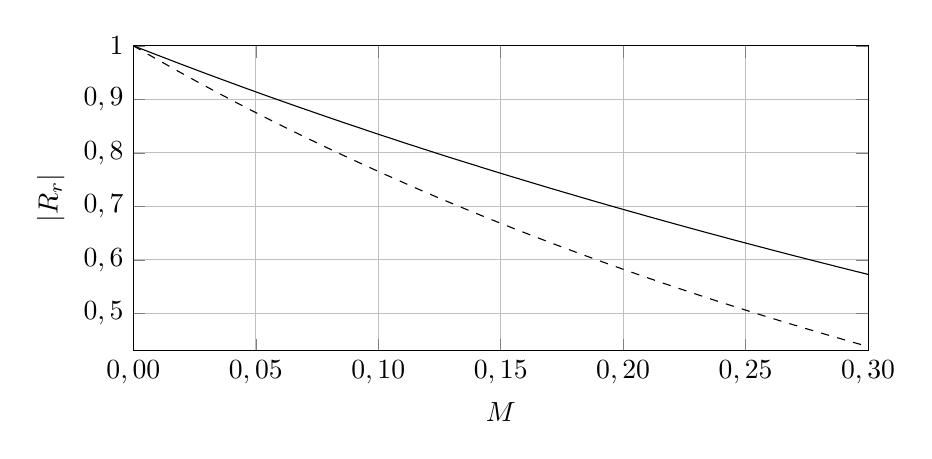
\begin{tikzpicture}
  \begin{axis}[
      %axis lines = left,
      xlabel = $M$,
      ylabel = $|R_{r}|$,
      width=0.9\textwidth,
      height=0.45\textwidth,
      ytick distance=0.1,
      x tick label style={
        /pgf/number format/.cd,
            fixed,
            fixed zerofill,
            precision=2, set decimal separator={,},
        /tikz/.cd
    },
    xmin=0,
    xmax=0.3,
    ymin=0.43,
    ymax=1,
    grid=major,
    y tick label style={/pgf/number format/.cd,%
          scaled y ticks = false,
          set decimal separator={,},
          fixed}
  ]
  \addplot [
      domain=0:0.3, 
      samples=100, 
      color=black
  ]
  {((1 - x)/(1 + x))^0.9};

  \addplot [
      domain=0:0.3, 
      samples=100, 
      color=black,
      dashed
  ]
  {((1 - x)/(1 + x))^1.333};
   
  \end{axis}
  \end{tikzpicture}
  \caption[Coeficiente de reflexão $|R_{r}|$ com escoamento sugado]{Resultado da magnitude do coeficiente de reflexão $|R_{r}|$ em relação ao Mach para baixas frequências com escoamento sugado. A linha contínua apresenta o cálculo obtido a partir do trabalho de \citeonline{davies1987} e a linha tracejada apresenta o resultado obtido a partir do trabalho de \citeonline{ingard1975}.}
  \label{fig:comp3}
\end{figure}

A Figura \ref{fig:comp3} mostra o gráfico resultante da equação \ref{eq:R_r_ingard} para os estudos de \citeonline{ingard1975} e  \citeonline{davies1987}. Pode-se perceber que $|R_{r}|$ decai de acordo com o aumento do Mach, em outras palavras, para baixas frequências, a onda plana possui maior facilidade de se radiar para o meio externo a medida que o Mach é aumentado. 


\begin{figure}[h!]
\centering
  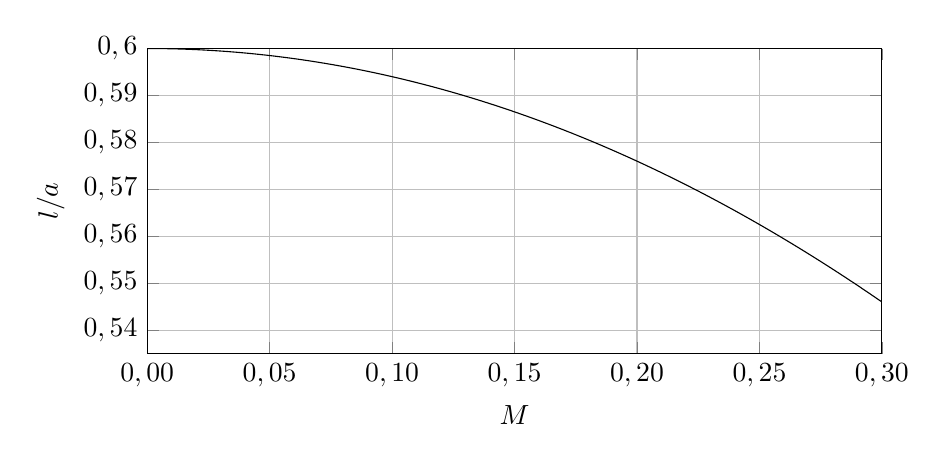
\begin{tikzpicture}
  \begin{axis}[
      %%axis lines = left,
      xlabel = $M$,
      ylabel = $l/a$,
      width=0.9\textwidth,
     height=0.45\textwidth,
      ytick distance=0.01,
       x tick label style={
        /pgf/number format/.cd,
            fixed,
            fixed zerofill,
            precision=2, set decimal separator={,},
        /tikz/.cd,
    },
    xmin=0,
    xmax=0.3,
    ymin=0.535,
    ymax=0.6,
    grid=major,
     y tick label style={/pgf/number format/.cd,%
          scaled y ticks = false,
          set decimal separator={,},
          fixed}
  ]
  %Below the red parabola is defined
  \addplot [
      domain=0:0.3, 
      samples=100, 
      color=black
  ]
  {0.6*(1 - x^2)};
   
  \end{axis}
  \end{tikzpicture}
  \caption[Coeficiente de correção da terminação $l/a$]{Resultado do coeficiente de correção da terminação $l/a$ em relação ao Mach para baixas frequências ($ka$ $<$ $0,25$), de acordo com \citeonline{davies1987}.}
  \label{fig:comp4}
\end{figure}

 A Figura \ref{fig:comp4} mostra o gráfico resultante da equação \ref{eq:l_M} e pode-se perceber que $l/a$ decai de acordo com o aumento do Mach, ou seja, para baixas frequências, o comprimento efetivo acustico do duto diminui a medida que o Mach do escoamento succionado é aumentado. Mesmo com esses coeficientes modelados com apoio de dados experimentais a literatura carece de informações sobre esses parâmetros para frequências mais altas ($ka$ $>$ $0,25$).


\section{Modelos Numéricos}

Já em relação a trabalhos envolvendo métodos numéricos, \citeonline{selamet2001wave} analisaram os coeficientes de reflexão e de terminação de dutos circulares com diferentes geometrias sem escoamento num contexto de ondas planas ($ka$ $<$ $1,8$). Para isso utilizaram método dos elementos de contorno e observaram que para diferentes razões de comprimento por raio de dutos não-flangeados, o comportamento acústico interno se diferencia muito pouco; no geral o coeficiente de reflexão, para dutos extendidos obliquamente a partir de uma parede rígida e infinita, decresce para altos números de $ka$ com relação aos extendidos de forma perpendicular; há uma redução significativa do coeficiente de reflexão para altos números de $ka$ em dutos terminados em forma de sino; dutos terminados com cavidade anular adiciona picos nos coeficientes de reflexão com relação aos não-flangeados.

Seguindo uma linha de análise semelhante, \citeonline{dalmont2001radiation} analisaram coeficientes de terminação de dutos circulares com diversas geometrias de terminação num contexto de ondas planas ($ka$ $<$ $1,8$), sobretudo as que são comumente encontradas em instrumentos de sopro. As análises foram feitas comparando-se resultados experimentais com resultados numéricos obtidos a partir dos métodos dos elementos finitos e elementos de contorno. A partir do ajuste dos modelos numéricos, derivaram modelos semi-empíricos simplificados para os coeficientes de reflexão encontrados nas geometrias estudadas. 

Tendo como motivação a validação do método de \textit{lattice} Boltzmann para problemas de acústica de dutos, \citeonline{da2006lattice} abordaram análises dos coeficientes de reflexão e de terminação de dutos circulares não flangeados, sem escoamento e focando ondas planas ($ka$ $<$ $1,8$). As boas correlações dos dados numéricos com os dados vigentes da teoria de \citeonline{levine1948radiation} mostram que o método é bastante útil para predizer fenômenos complexos envolvendo acústica de dutos.

Complementando o trabalho anterior, \citeonline{da2009sound} investigaram os coeficientes de reflexão e de terminação de dutos circulares com terminações de corneta e com escoamento subsônico. Para isso implementaram o modelo usando o método de \textit{lattice} Boltzmann com condições de contorno absorventes, axissimetria de acordo com o trabalho de \citeonline{reis2007} e paredes curvas para a consolidação das terminações em cornetas. Com esse trabalho foram validados os resultados de \citeonline{munt1990acoustic} e \citeonline{allam2006investigation} além de mostrar que na presença de cornetas o coeficiente de reflexão aumenta bastante no pico associado ao número de Strouhal $St \approx \frac{\pi}{2}$\simbolo{$St$}{Número de Strouhal}. Tal fato é aderente aos vários trabalhos que abordam o escoamento de exaustão e é explicado pelo fato de valores maiores do que a unidade para a magnitude do coeficiente de reflexão podem ser encontrados tanto em dutos não-flangeados quanto cornetas. No entanto, no caso das cornetas, este aumento é consideravelmente maior devido a indução de vorticidade causada pela terminação circular. Além disso, os resultados observados sugerem que a região de Strouhal $St \approx \frac{\pi}{2}$ acontecem quando o período do campo acústico interno conicide com o tempo necessário para que um vórtice propague a distância equivalente a um raio de corneta.

\citeonline{silva2012approximate} usaram o método de elementos de contorno para analisar a influência do raio de uma terminação flangeada no comportamento do coeficiente de reflexão de dutos circulares na ausência de escoamento. Para tanto validaram o modelo com os resultados de \citeonline{levine1948radiation}, dutos não flangeados, e de \citeonline{nomura1960}, dutos flangeados circulamente. Como resultado da análise propuseram expressões aproximadas para o cálculo dos coeficientes de reflexão e de terminação.
